\documentclass[11pt, a4paper]{article}

% --- Packages ---
\usepackage[utf8]{inputenc}
\usepackage[T1]{fontenc}
\usepackage[french]{babel}
\usepackage[margin=2.5cm, top=3.5cm, headheight=30pt, headsep=1cm]{geometry} 
\usepackage{graphicx}
\usepackage{svg}
\usepackage{xcolor}
\usepackage{hyperref}
\usepackage{float}
\usepackage{titlesec}
\usepackage{fancyhdr}
\usepackage[most]{tcolorbox}
\usepackage{booktabs}
\usepackage{caption}
\usepackage{subcaption}
\usepackage{parskip} % Espacement intelligent entre les paragraphes (évite les gros blocs compacts)
\usepackage{enumitem} % Personnalisation des listes à puces

% --- Couleurs du Projet ---
\definecolor{primary}{RGB}{30, 61, 89} % Bleu profond
\definecolor{secondary}{RGB}{255, 107, 107} % Rouge clair
\definecolor{accent}{RGB}{245, 245, 245} % Gris clair fond
\definecolor{success}{RGB}{39, 174, 96} % Vert validation

% --- Configuration des Hyperliens ---
\hypersetup{
    colorlinks=true,
    linkcolor=primary,
    filecolor=secondary,      
    urlcolor=blue,
    pdftitle={Rapport Technique Détaillé - Detect Football Talents},
}

% --- Style des Titres ---
\titleformat{\section}
  {\normalfont\Large\bfseries\color{primary}}{\thesection}{1em}{}[{\color{primary}\titlerule[1.5pt]}]
\titleformat{\subsection}
  {\normalfont\large\bfseries\color{primary!80!black}}{\thesubsection}{1em}{}
\titleformat{\subsubsection}
  {\normalfont\normalsize\bfseries\color{primary!60!black}}{\thesubsubsection}{1em}{}

% --- En-tête et Pied-de-page ---
\pagestyle{fancy}
\fancyhf{}
\fancyhead[L]{\textcolor{primary}{\textbf{Detect-Football-Talents}}}
\fancyhead[R]{\nouppercase{\leftmark}}
\fancyfoot[C]{\thepage}
\renewcommand{\headrulewidth}{0.6pt}
\renewcommand{\footrulewidth}{0.6pt}

\begin{document}

% ==================== PAGE DE GARDE ====================
\begin{titlepage}
    \centering
    \vspace*{1.5cm}
    
    {\Huge \textbf{\textcolor{primary}{Rapport Technique Détaillé}} \par}
    \vspace{0.5cm}
    {\LARGE \textbf{Projet : Detect-Football-Talents} \par}
    
    \vspace{1.5cm}
    
    \begin{tcolorbox}[colback=primary!5!white,colframe=primary,arc=5pt,boxrule=1.5pt]
        \centering
        \large\textbf{Conception et Réalisation sur 4 Semaines} \\
        \vspace{0.3cm}
        \normalsize Ce rapport documente en profondeur l'architecture, le développement SQL/Python et l'intégration continue via Airflow d'un écosystème Big Data orienté vers la détection d'opportunités sur le marché du football.
    \end{tcolorbox}
    
    \vspace{1.5cm}
    
    {\Large \textbf{Sommaire des Réalisations} \par}
    \vspace{0.5cm}
    \begin{tabular}{rl}
        \textbf{Semaine 1:} & Définition du besoin, Modélisation Conceptuelle (MCD) et sources \\
        \textbf{Semaine 2:} & Schéma en étoile (PostgreSQL), Scripts de création et intégrité \\
        \textbf{Semaine 3:} & Algorithmique SQL, KPIs décisionnels, Streamlit Dashboard \\
        \textbf{Semaine 4:} & Industrialisation, ETL via Apache Airflow et conteneurs Docker \\
    \end{tabular}
    
    \vfill
    
    % --- ZONE INFORMATIONS PERSONNELLES ---
    \begin{tcolorbox}[colback=white,colframe=primary!40,arc=5pt,boxrule=1pt,width=0.9\textwidth,halign=left]
        \normalsize \textcolor{primary}{\textbf{\textsf{ INFORMATIONS PERSONNELLES}}} \\[0.3cm]
        \renewcommand{\arraystretch}{1.5}
        \begin{tabular}{ll}
            \textbf{Nom \& Prénom} & : ............................................................................................... \\
            \textbf{Classe / Filière} & : ............................................................................................... \\
            \textbf{Année Scolaire} & : ............................................................................................... \\
            \textbf{Professeur Encadrant} & : ............................................................................................... \\
        \end{tabular}
    \end{tcolorbox}
    
    \vspace{1.5cm}
    {\large \today \par}
\end{titlepage}

% ==================== SOMMAIRE ====================
\tableofcontents
\newpage

% ==================== INTRODUCTION ====================
\section{Aperçu et Contexte du Projet}

Dans le cadre de notre apprentissage réparti sur \textbf{quatre semaines de classe}, nous avons mené de bout en bout le projet \textbf{Detect-Football-Talents}. Face à un marché des transferts footballistique régi par la notoriété médiatique, ce produit a pour vocation de déceler la \og valeur réelle \fg{} des sportifs grâce à une approche purement analytique (Expected Goals, efficacité, création d'occasions).

L'élaboration de ce système s'écarte du simple tableur : elle plonge directement dans les standards de l'Ingénierie des Données (\textit{Data Engineering}). 
Des fondations relationnelles sous PostgreSQL à l'orchestration des données via Docker et Apache Airflow, chaque chapitre de ce rapport justifie les choix architecturaux qui font de ce projet une solution autonome, robuste et décisionnelle.

% ==================== SEMAINE 1 ====================
\section{Semaine 1 : Lancement, Spécifications et Schéma Directeur}

La première semaine ne fut pas consacrée au code aveugle, mais au balisage de notre cadre analytique et à la chasse d'une donnée d'exception capable d'alimenter nos futurs calculs.

\subsection{Sélection et Intelligence des Sources (Jours 1-2)}

La problématique étant d'observer l'efficacité au-delà de la "chance", nous avions besoin de variables avancées introuvables dans la statistique traditionnelle. Nous avons croisé deux sources majeures :
\begin{itemize}[label=\textcolor{primary}{$\bullet$}, leftmargin=*]
    \item \textbf{Understat :} L'extraction de ce portail offre la maîtrise de probabilités pures. L'obtention de métriques telles que les \textit{Expected Goals (xG)} (buts statistiquement attendus selon la position) et les \textit{Expected Assists (xA)} certifie la pertinence prédictive de notre plateforme.
    \item \textbf{SofaScore :} L'agrégation de ce service a servi à relier chaque profil de joueur à des métadonnées fiables (Âge, Club, Matchs professionnels joués, Pied favori).
\end{itemize}

Ce croisement permet de répondre, sans ambiguïté analytique, à notre \textbf{test de la donnée} et autorise un rendu qualitatif.

\subsection{Nettoyage Préparatoire et Modélisation en Étoile (Jours 3-5)}

\paragraph{Aptitude et Tolérance de la Donnée :}
Lors de l'export JSON des plateformes, un flux brut nécessite une normalisation. Avec des librairies Python telles que \texttt{Pandas}, des actions express de curation ont été entreprises :
\begin{itemize}[label=\textcolor{primary}{\checkmark}]
    \item Typage fort des variables (Les métriques Per 90 en format \texttt{Float}, les âges en \texttt{Int}).
    \item Retrait des doublons et impositions de clés d'identifications (\texttt{id}) uniques pour le joueur et le club affecté afin de pré-contraindre nos futurs imports relationnels.
\end{itemize}

\paragraph{L'Architecture du Modèle Conceptuel (MCD) :}
Afin d'optimiser radicalement la vitesse nos tableaux de bords, nous n'avons pas choisi une division standard en 3\textsuperscript{ème} forme normale classique. Nous avons opté un typage de Data Warehouse de \textbf{Modèle en Étoile (\textit{Star Schema})} organisé autour :
\begin{enumerate}
    \item \textbf{D'une Table de Faits centrale :} Elle contient toutes les valeurs continues observables (Les tirs, les buts, le nombre de Key Passes).
    \item \textbf{De ses Dimensions :} Qui sont les axes subjectifs de l'analyse (Qui a frappé ? Dans quelle ligue ? À quelle période de la saison ?).
\end{enumerate}

\begin{figure}[H]
    \centering
    \includesvg[width=0.9\textwidth, inkscapelatex=false]{images_Football_Talents/erd_star_schema_fixed}
    \caption{Diagramme et formalisation de notre Modèle Décisionnel en Étoile}
\end{figure}

\begin{tcolorbox}[colback=success!10,colframe=success!80!black,title=\textbf{Bilan et Validation - Semaine 1}]
    La fondation est documentée. Les exigences pédagogiques (Dictionnaire des données, formulation claire de la question décisionnelle et élaboration complète du modèle avec 4 dimensions fortes pour la jointure) ont été réalisées.
\end{tcolorbox}


% ==================== SEMAINE 2 ====================
\section{Semaine 2 : L'Écosystème Physique et Contraintes (PostgreSQL)}

Durant la seconde étape, le schéma conceptuel a basculé vers le monde physique (SQL / DDL). L'objectif était de bâtir un environnement infaillible aux incohérences d'insertion de notre moteur de récupération.

\subsection{Défintion des tables et Normalisation Stricte}

Une grande partie du mérite revient au script robuste de mise en base. Le modèle devant traiter des milliers de lignes mises à jour chaques semaines, plusieurs logiques de stockage furent créées de concert avec **PostgreSQL** :
\begin{itemize}[label=\textcolor{primary}{$\bullet$}, leftmargin=*]
    \item \textbf{Cohérence de la mémoire :} Les indices de prédictions ($xG$) ont été fixés à \texttt{DECIMAL(10,2)} pour économiser de l'espace tout en obtenant deux chiffres de précision, cruciaux pour un ratio.
    \item \textbf{Intégrité des Liens :} Chaque création de métrique exige l'absolue définition de \texttt{FOREIGN KEY} pointant vers les tables Joueurs et Équipes via \texttt{ON DELETE CASCADE} le cas échéant.
\end{itemize}

L'existence et les types ont été vérifiées physiquement au travers de l'éditeur *pgAdmin* :

\begin{figure}[H]
    \centering
    \begin{minipage}{0.45\textwidth}
        \centering
        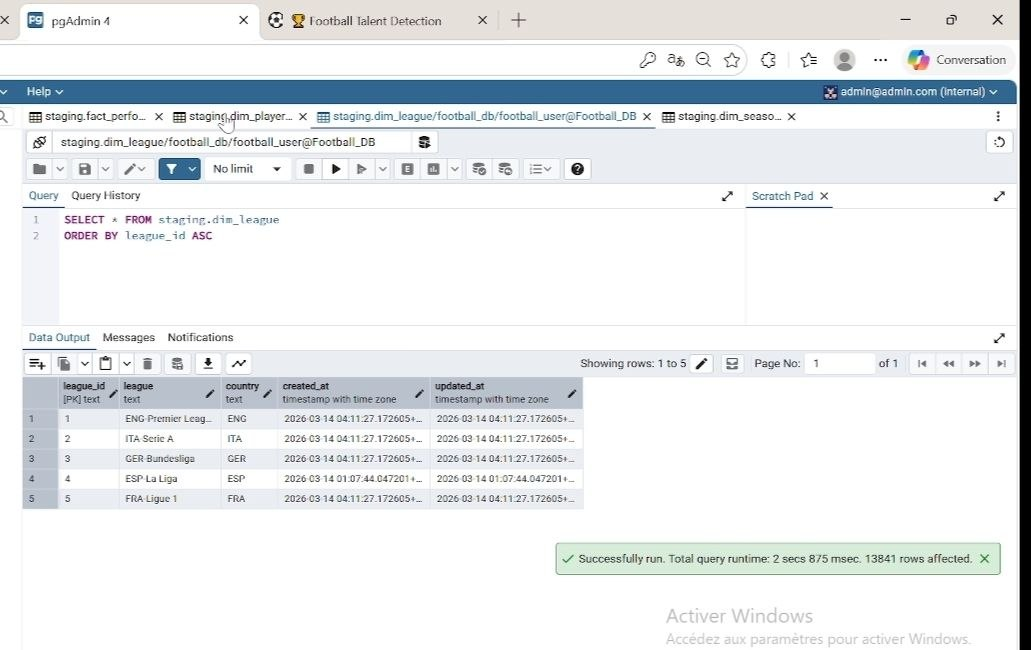
\includegraphics[width=\linewidth]{images_Football_Talents/dim_league.jpg}
        \caption{Formatage et typage de \texttt{dim\_league}}
    \end{minipage} \hfill
    \begin{minipage}{0.45\textwidth}
        \centering
        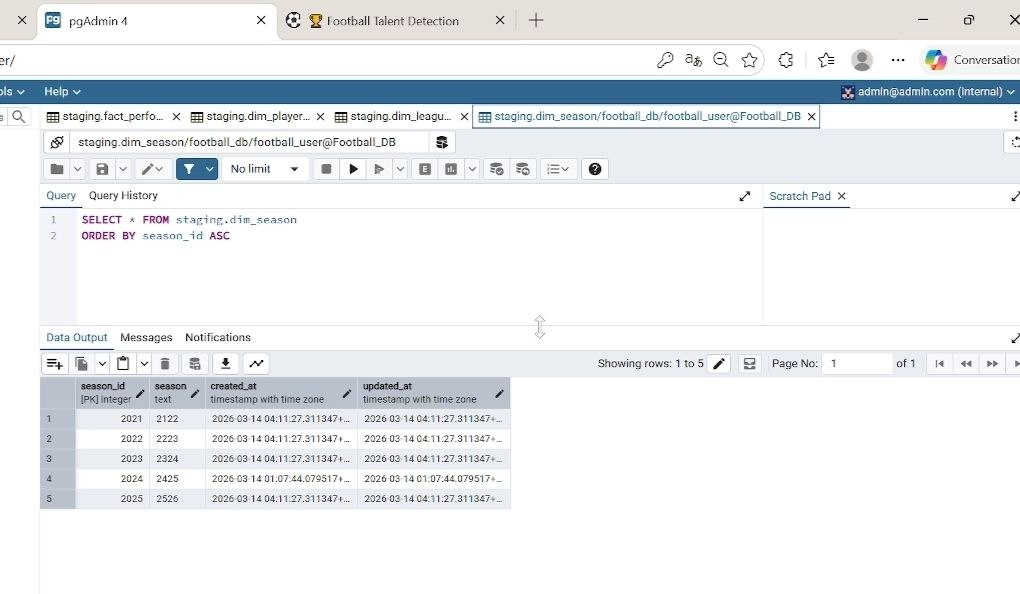
\includegraphics[width=\linewidth]{images_Football_Talents/dim_season.jpg}
        \caption{Création de de la table temps \texttt{dim\_season}}
    \end{minipage}
    
    \vspace{0.6cm}
    
    \begin{minipage}{0.45\textwidth}
        \centering
        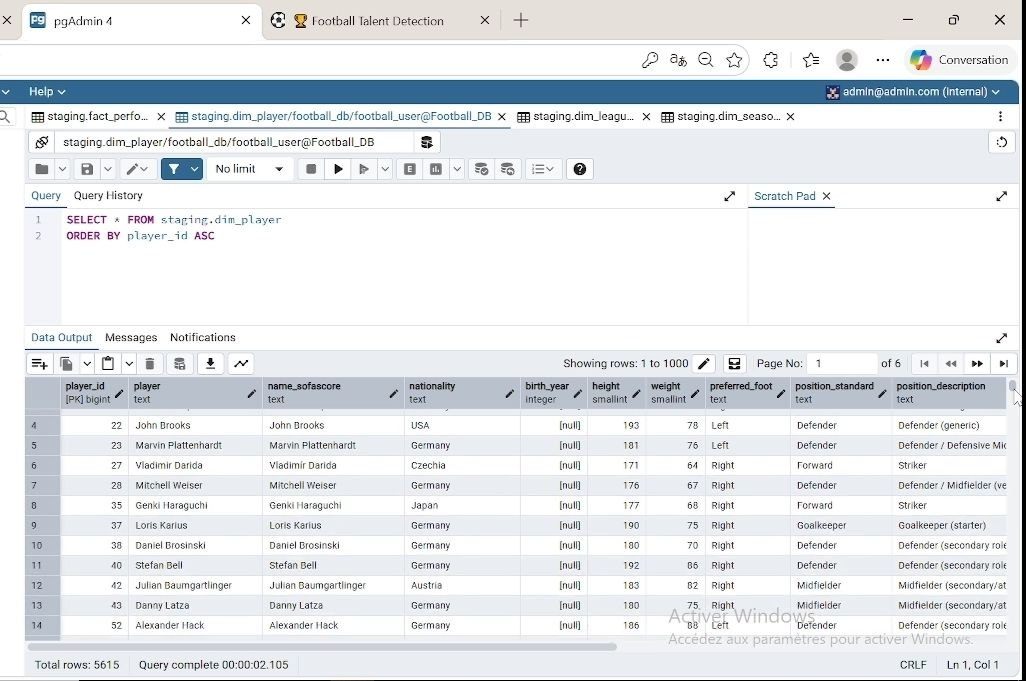
\includegraphics[width=\linewidth]{images_Football_Talents/dim_player.jpg}
        \caption{Gestion de l'historique joueur \texttt{dim\_player}}
    \end{minipage} \hfill
    \begin{minipage}{0.45\textwidth}
        \centering
        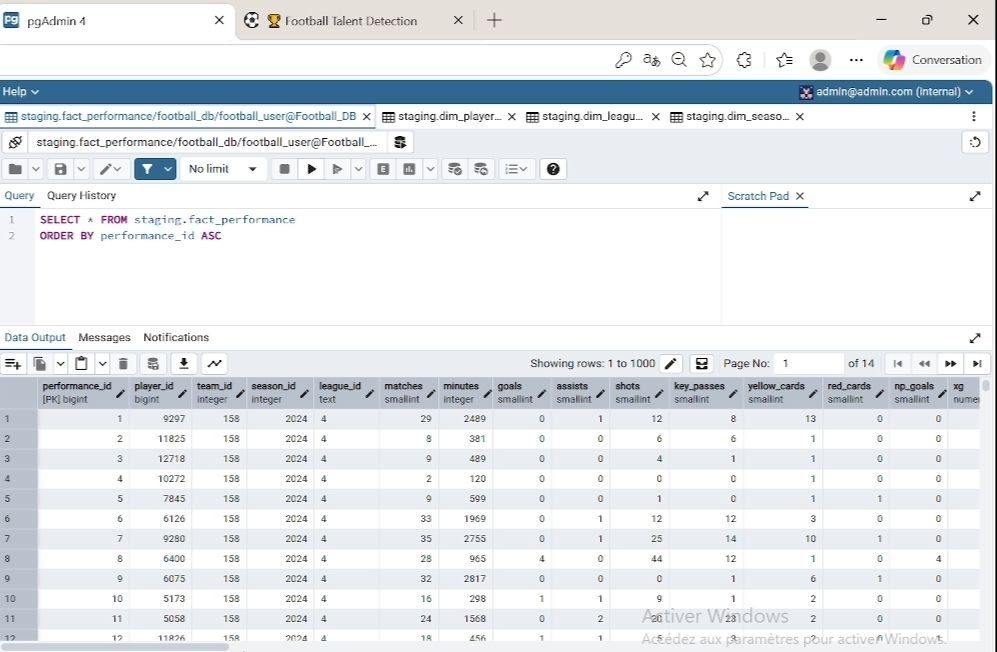
\includegraphics[width=\linewidth]{images_Football_Talents/dim_performance.jpg}
        \caption{Aggrégat strict de notre table de Faits}
    \end{minipage}
\end{figure}

\subsection{Le Choc du Chargement : Insertion Incrémentale et Requêtes de validations}

Face aux données footballistiques où le total d'un joueur change à chaque rencontre professionnelle (Ex: passage de 2 buts à 3), un simple ordre \texttt{INSERT} allait inexorablement créer des doublons toxiques pour l'agrégation finale. 

\paragraph{Solutions d'insertion (UPSERT) :}
L'adoption de clauses \texttt{ON CONFLICT (id) DO UPDATE} nous a permis de repérer si le joueur existait déjà. S'il existe, seule sa colonne des données actualisées des buts/matchs remplace celle de l'enregistrement, assurant un pipeline propre et continu.

Une fois complétée, nous avons satisfait la commande obligatoire des cinq requêtes test allant du regroupement \texttt{GROUP BY} aux calculs inter-entités \texttt{AVG()}, garantissant alors l'exactitude de nos montages. Par exemple, isoler le temps de jeu complet d'une équipe donnée permet de vérifier sans erreur que notre liaison en clé étrangère fonctionne à grande échelle.

\begin{tcolorbox}[colback=success!10,colframe=success!80!black,title=\textbf{Bilan et Validation - Semaine 2}]
    La couche de persistance fonctionne à la perfection. La table garantit des données non redondantes, le choix des types est optimisé. La structure "Étoile" permet maintenant la jonction instantanée à bas coût transactionnel en vue de la modélisation à suivre.
\end{tcolorbox}


% ==================== SEMAINE 3 ====================
\section{Semaine 3 : Moteur Algorithmique et Streamlit BI}

Une base pleine de données n'a qu'un intérêt consultatif. L’objectif a été de greffer des logiques de Data Science en SQL et d'offrir le tout à un directeur sportif grâce à un outil interactif esthétique (Front-End). 

\subsection{L'Architecture des Vues et KPIs Complexifiés}

Afin de préserver l'interface Python, les calculs mathématiques pointus sont embarqués directement sous PostgreSQL (Common Table Expressions - CTE et vues analytiques).
Nous avons conceptualisé \textbf{5 KPIs fondateurs} et \textbf{2 filtres opérationnels} :
\begin{itemize}[label=\textcolor{primary}{$\triangleright$}]
    \item \textbf{Efficacité Brute (Goals - xG) :} Capacité exceptionnelle du joueur à marquer même dans des situations très désavantageuses.
    \item \textbf{Indice d'orientation (xA per 90) :} La part statistique de bons ballons servis par minutes (normalisé sur la rencontre de 90m).
    \item \textbf{Filtrage de Robustesse (HAVING minutes > X) :} Écrêtage statistique pour supprimer les excellents ratios d'un joueur n'ayant joué qu'une vingtaine de minutes dans l'année.
\end{itemize}

\subsection{Le Tableau de Bord Décisionnel (Streamlit)}

Le produit est porté par la technologie \textbf{Streamlit} où le soin du design a rendu la donnée accessible. La sidebar de gauche inclut une batterie de curseurs (Équipes, Championnats, Limite d'âge sur le vivier) permettant d'obtenir le calcul instantané des vues configurées précédemment à l'étape SQL.

\begin{figure}[H]
    \centering
    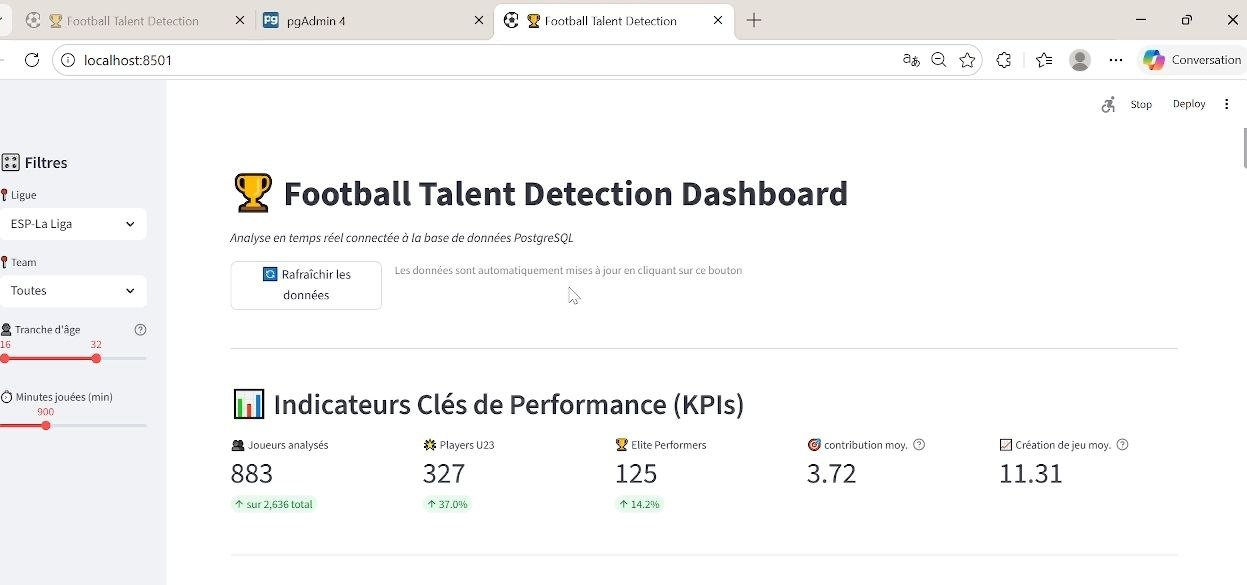
\includegraphics[width=0.85\textwidth]{images_Football_Talents/kpi_filtres.jpg}
    \caption{Dynamisme des KPIs via les sliders analytiques en temps réel}
\end{figure}

Les observations métier (scouting) changent drastiquement selon le positionnement de l'individu, les "Dashboards" ont par conséquent été cloisonnées :

\begin{figure}[H]
    \centering
    \begin{minipage}{0.48\textwidth}
        \centering
        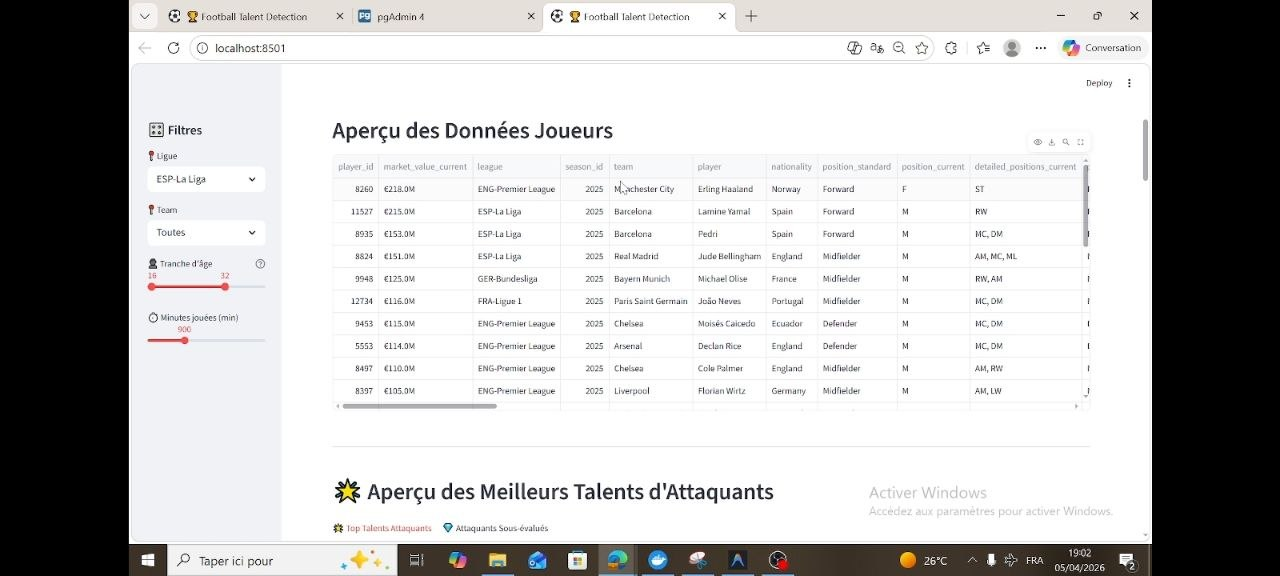
\includegraphics[width=\linewidth]{images_Football_Talents/apercu_joueurs.jpg}
        \caption{Aperçu et métriques centrales}
    \end{minipage}\hfill
    \begin{minipage}{0.48\textwidth}
        \centering
        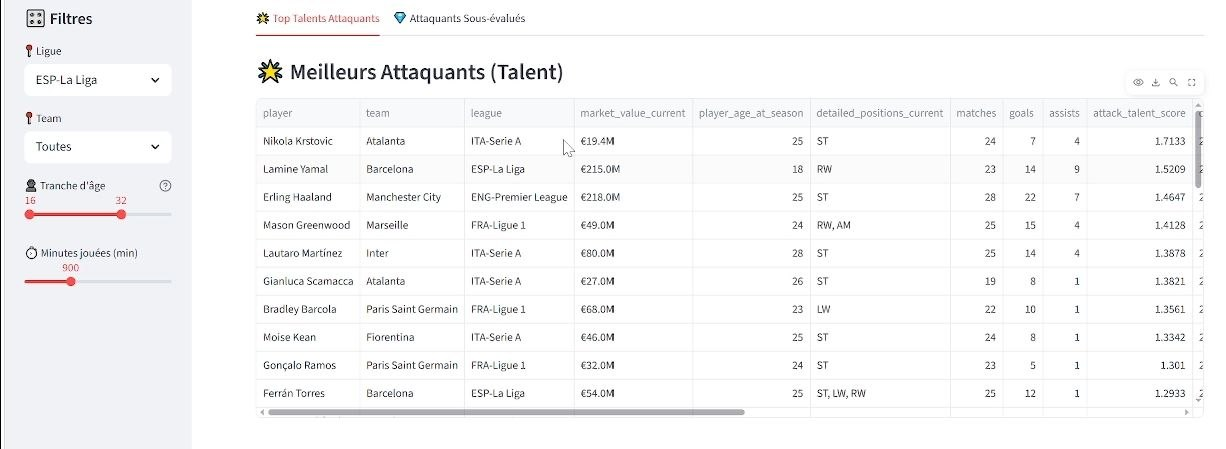
\includegraphics[width=\linewidth]{images_Football_Talents/apercu_attaquants.jpg}
        \caption{Secteur Attaquant et finition face au but}
    \end{minipage}
    
    \vspace{0.4cm}
    \centering
    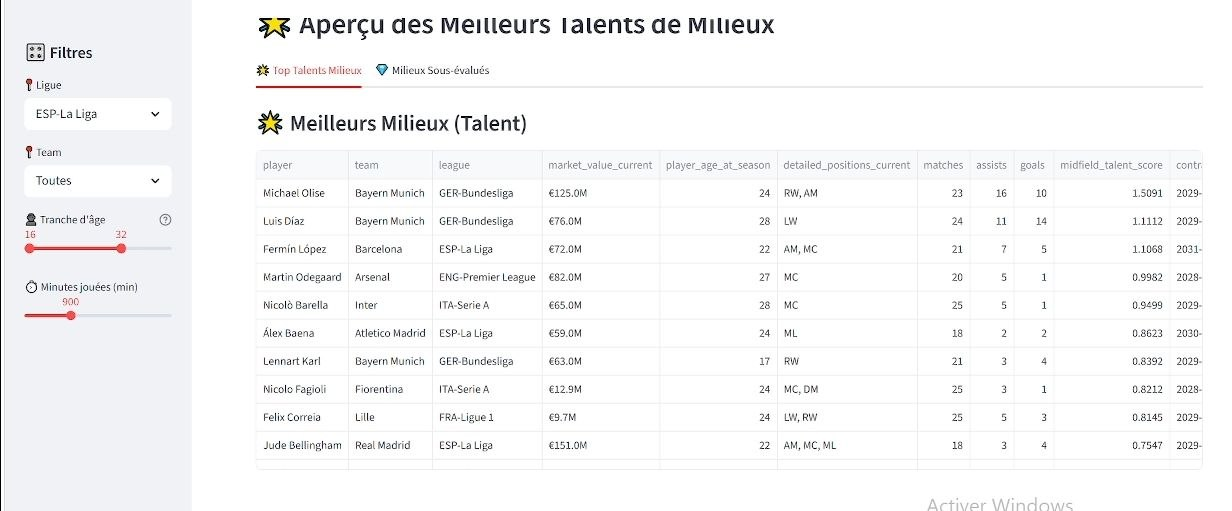
\includegraphics[width=0.7\textwidth]{images_Football_Talents/apercu_milieux.jpg}
    \caption{Secteur Milieu et Créateur d'espace (\textit{Playmaking})}
\end{figure}

De surcroît, la librairie \texttt{Plotly} insuffle de l'interactivité aux corrélations graphiques pour repérer les anomalies "Outliers", c'est-à-dire le type même d'une pépite footballistique que l'on recherche où ses indices xG et buts explosent littéralement.

\begin{figure}[H]
    \centering
    \begin{minipage}{0.48\textwidth}
        \centering
        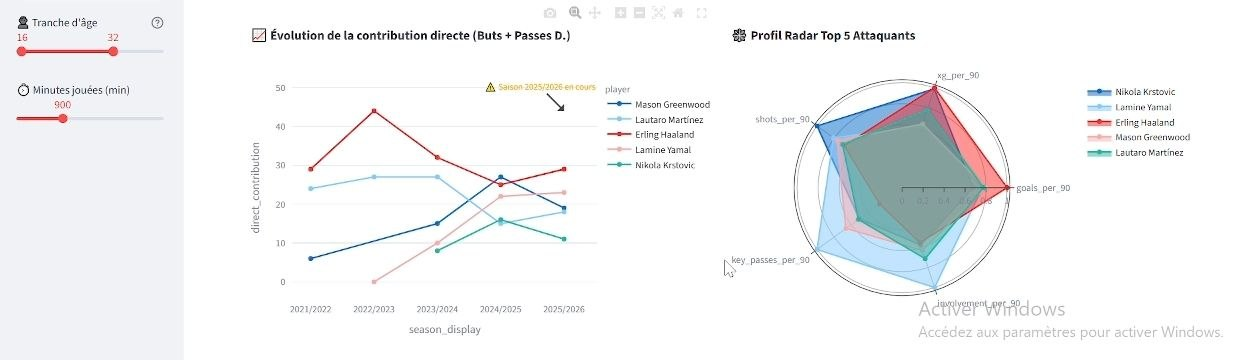
\includegraphics[width=\linewidth]{images_Football_Talents/graphes_attaquants.jpg}
        \caption{Cartographie et dispersion offensive}
    \end{minipage}\hfill
    \begin{minipage}{0.48\textwidth}
        \centering
        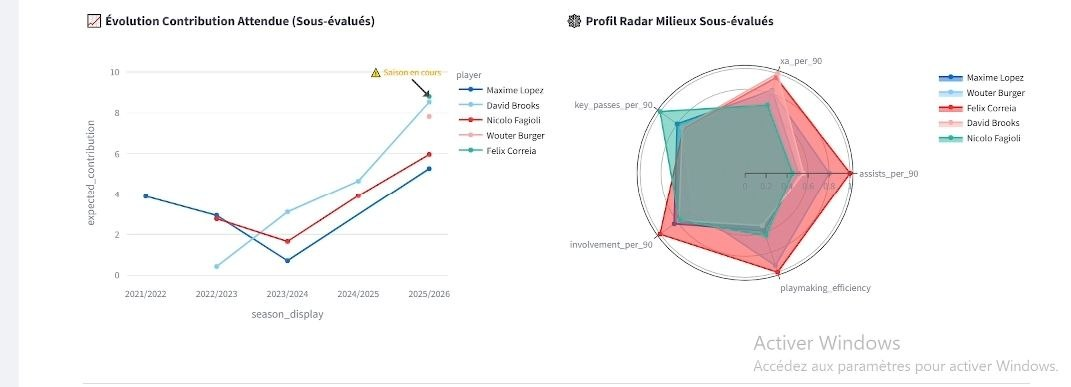
\includegraphics[width=\linewidth]{images_Football_Talents/graphes_milieux.jpg}
        \caption{Créativité vs minutes disputées}
    \end{minipage}
\end{figure}

\begin{tcolorbox}[colback=success!10,colframe=success!80!black,title=\textbf{Bilan et Validation - Semaine 3}]
    Le seuil de présentation est atteint. La construction logicielle complexe (Requêtes Imbriquées PostgreSQL) liée de manière transparente au code asynchrone Streamlit transforme ce qui était auparavant un fichier "inertes" en un véritable produit technologique SaaS orienté décision.
\end{tcolorbox}


% ==================== SEMAINE 4 ====================
\section{Semaine 4 : Airflow, Déploiement et Pitch Dirigeant}

Le dernier volet consiste en l'intégration continue (\textit{DataOps CI/CD}) afin que cet outil vive seul de manière cyclique sans surveillance active. L'automatisation du flux d'information (ETL), autrefois géré via l'exécution des scripts à la main, est désormais orchestrée.

\subsection{Cloud local Docker et Séquençage via (Airflow)}

Le système informatique est figé dans une architecture sécurisée \textbf{Docker Compose} : notre instance PostgreSQL cohabite en transparence réseau absolue avec \textbf{Apache Airflow}. Concrètement, nous avons codé le séquençage d’information via de Graphes Orientés (DAG) programmées :
\begin{itemize}[label=\textcolor{primary}{$\bullet$}, leftmargin=*]
    \item Un DAG massif appelé (\texttt{football\_etl\_all\_seasons}) pour charger depuis ses origines web tout l'historique non digéré à l'initialisation du premier serveur.
    \item Un DAG d'incrémentation légère (\texttt{football\_etl\_weekly\_update}), exécuté selon une commande automatique "CRON", récupérant pour sa part la simple évolution constatée lors des week-ends sportifs de la saison en cours.
\end{itemize}

\begin{figure}[H]
    \centering
    % Remarque : Taille réduite à 0.75 par rapport à texte (contre un full textwidth auparavant) pour l'esthétique demandée.
    \includesvg[width=0.78\textwidth, inkscapelatex=false]{images_Football_Talents/project_workflow_stack_technique}
    \caption{Architecture Détaillée du Flux Automatisé et Orchestrations Airflow}
\end{figure}

\begin{figure}[H]
    \centering
    \begin{minipage}{0.32\textwidth}
        \centering
        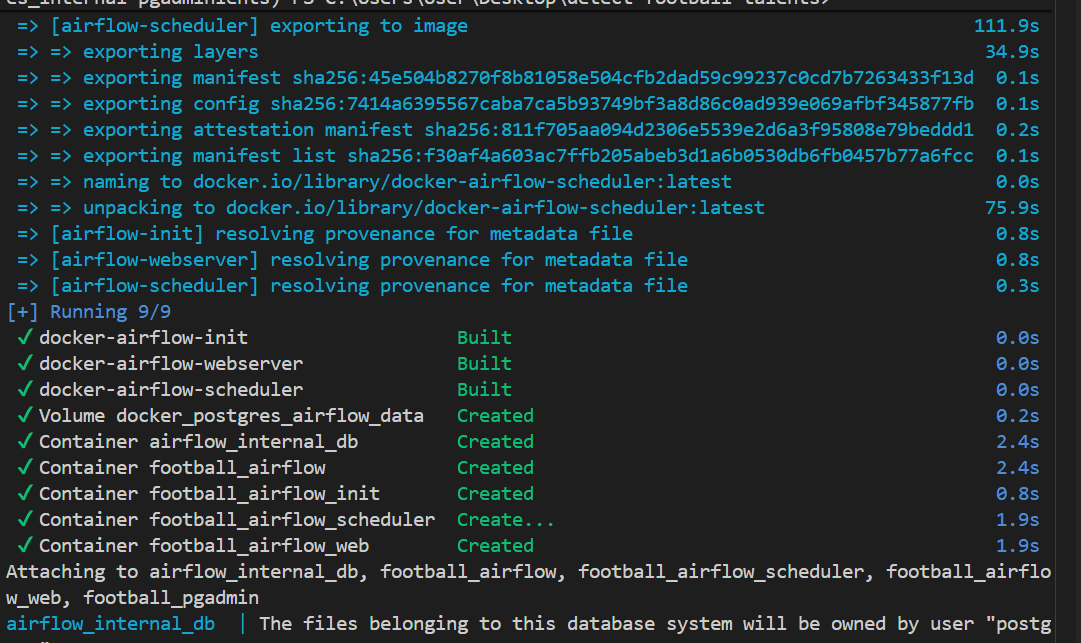
\includegraphics[width=\linewidth]{images_Football_Talents/building_containers.PNG}
        \caption{Mise en conformité Docker}
    \end{minipage}\hfill
    \begin{minipage}{0.32\textwidth}
        \centering
        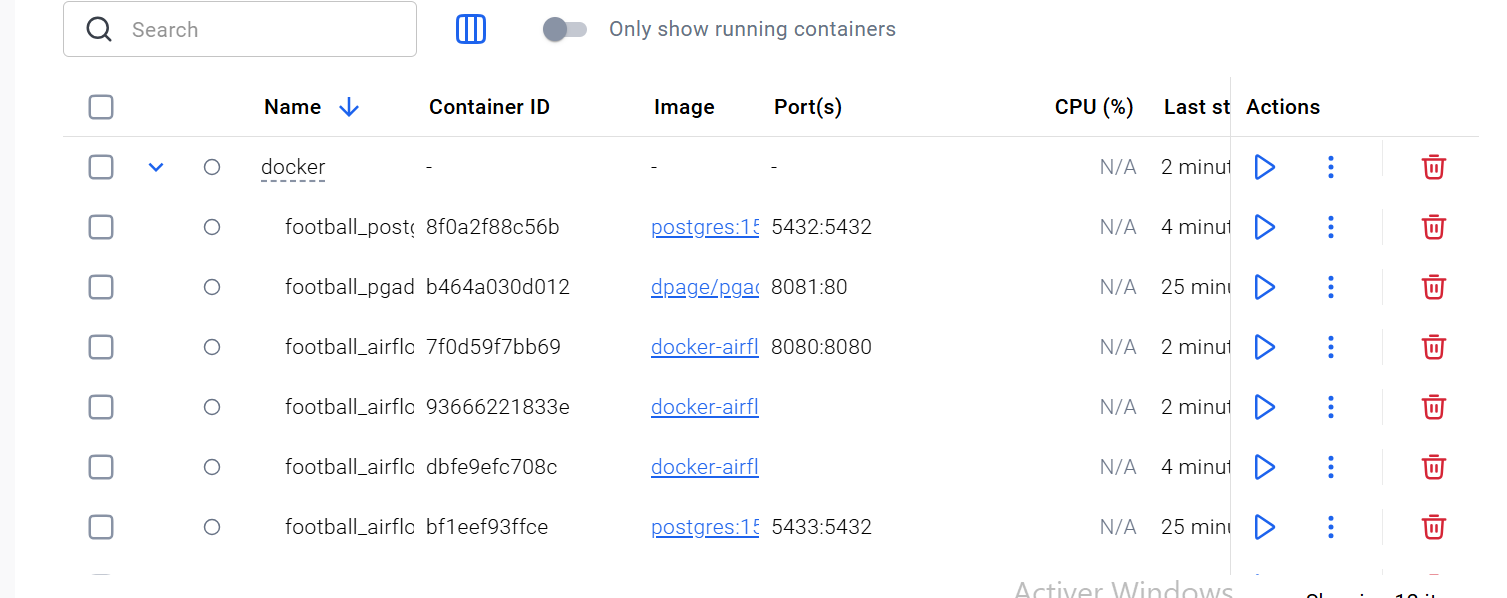
\includegraphics[width=\linewidth]{images_Football_Talents/docker_contaniers.PNG}
        \caption{Volumes et Conteneurs actifs}
    \end{minipage}\hfill
    \begin{minipage}{0.32\textwidth}
        \centering
        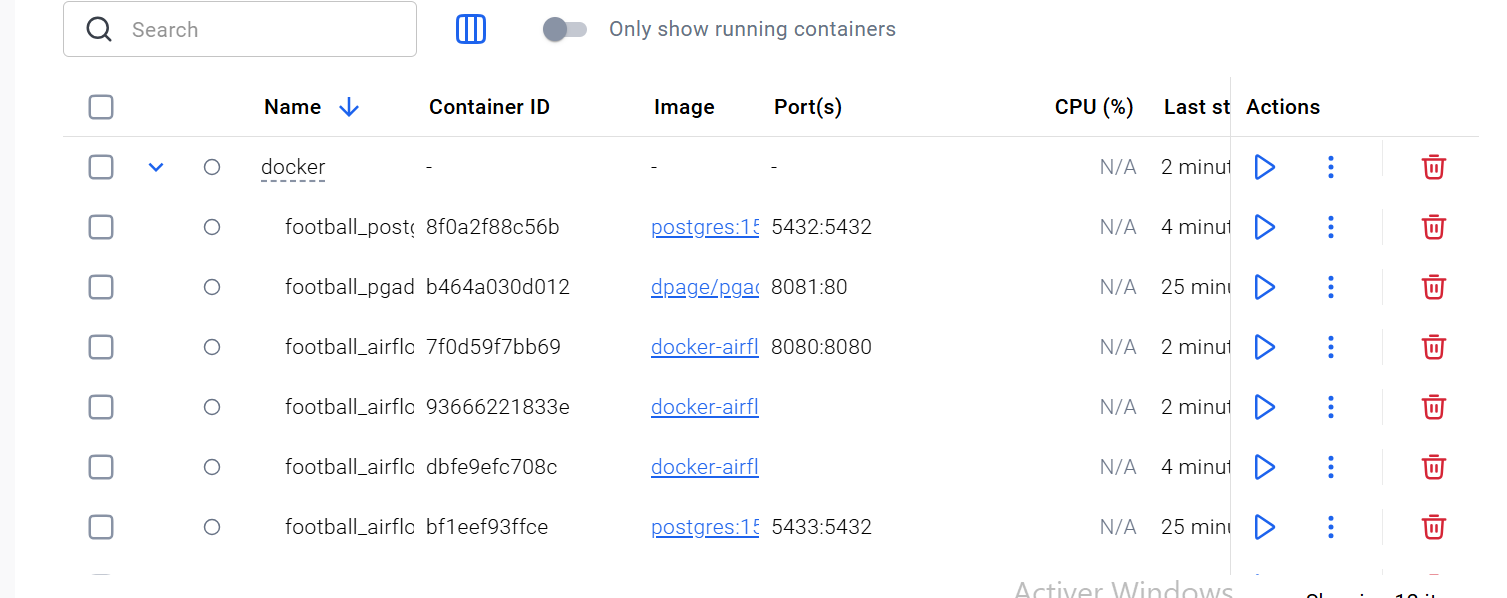
\includegraphics[width=\linewidth]{images_Football_Talents/pgadmin_server.PNG}
        \caption{Écran d'observation serveur}
    \end{minipage}
\end{figure}

\subsection{La Livraison de la Valeur et le Pitch}

L'évaluation de clôture n'exigeait plus du code, mais de l'argumentation. Dans un "Pitch de Direction" calibré pour le monde réel, nous avons défendu un ciblage prévisionnel de joueur au profit d'une recommandation statée par nos calculs. C'est l'essence même de ce projet : faire valoir que la Data outrepasse le prestige lorsqu'il s'agit de repérer un athlète d'exception à petit budget.

\begin{figure}[H]
    \centering
    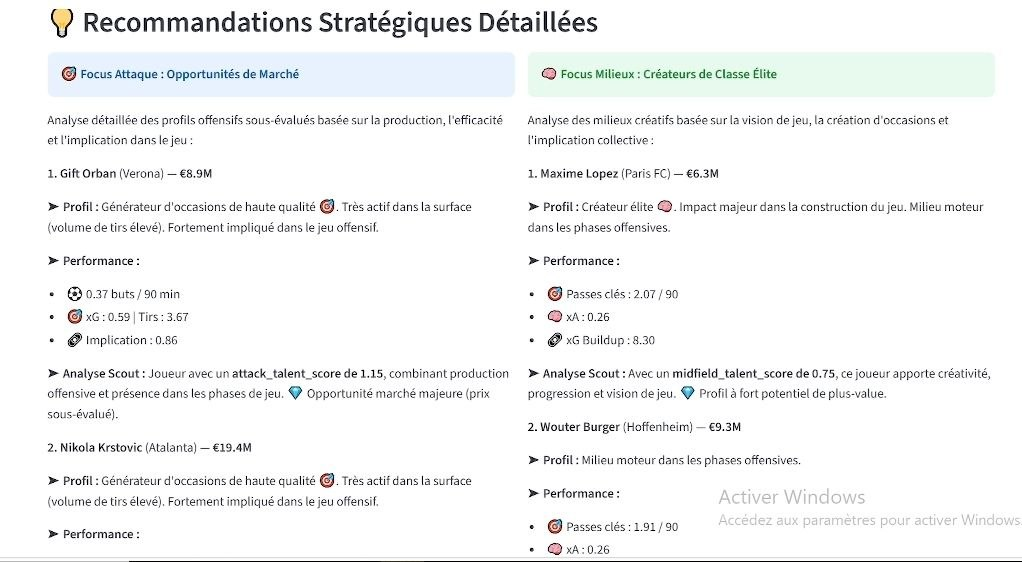
\includegraphics[width=0.85\textwidth]{images_Football_Talents/recommendations_strategiques.jpg}
    \caption{Extrait de Document de Synthèse orienté pour une Direction Sportive}
\end{figure}

\begin{tcolorbox}[colback=success!10,colframe=success!80!black,title=\textbf{Bilan et Validation - Semaine 4}]
    L'industrialisation (Production-ready) scelle le destin du projet. Airflow exécute avec cadence les chargements pendant que Docker préserve la sécurité de l'environnement de pannes locales. La justification managériale clôt ce cours en beauté.
\end{tcolorbox}


% ==================== CONCLUSION ====================
\section{Conclusion Générale de la Formation}

Au terme du mois d'apprentissage, l’application de Data Intelligence \textbf{Detect-Football-Talents} transcende le statut de simple exercice en classe : c'est un produit bout en bout accompli, orchestré, résilient au temps, reposant sur une architecture normalisée pérenne.

La maîtrise combinée des écosystèmes Extract/Transform (\texttt{Pandas}, APIs), de la persistance relationnelle logicielle robuste (\texttt{PostgresSQL}), du rendu pré-décisionnel visuel de très haut niveau (\texttt{Streamlit}) et de son automatisation imperturbable (\texttt{Docker, Airflow}) concrétisent pleinement sur toutes les dimensions les exigences fondamentales du diplôme de Data Engineering et d'analyste de l’information.

\end{document}
